\documentclass[bachelor, och, pract]{SCWorks}
\usepackage[T2A]{fontenc}
\usepackage[utf8]{inputenc}

\usepackage{graphicx}
\usepackage[sort,compress]{cite}
\usepackage{amsmath}
\usepackage{amssymb}
\usepackage{amsthm}
\usepackage{fancyvrb}
\usepackage{longtable}
\usepackage{listings}
\usepackage{array}
\usepackage{tikz}
\usepackage{pgfplots}
\usepackage[english,russian]{babel}

\usepackage{listings}
\usepackage{listings-golang}

\lstset{language=Swift}
\lstset{numbers = left}
\lstset{numberstyle = \tiny}
\lstset{basicstyle=\small}
\lstset{breaklines=true}
\lstset{extendedchars=true}
\lstset{breakatwhitespace=true}

\usepackage[colorlinks=true]{hyperref}

\newcommand{\eqdef}{\stackrel {\rm def}{=}}



\begin{document}
	
	% Кафедра (в родительном падеже)
	\chair{математической кибернетики и компьютерных наук}
	
	% Тема работы
	\title{Построение архитектуры  ETL процесса и ее программная реализация}
	
	% Курс
	\course{4}
	
	% Группа
	\group{411}
	
	% Факультет (в родительном падеже) (по умолчанию "факультета КНиИТ")
	%\department{факультета КНиИТ}
	
	% Специальность/направление код - наименование
	\napravlenie{02.03.02 "--- Фундаментальная информатика и информационные технологии}
	
	% Фамилия, имя, отчество в родительном падеже
	\author{Вязкова Андрея Андреевича}
	
	% Заведующий кафедрой
	\chtitle{к.\,ф.-м.\,н.} % степень, звание
	\chname{А.\,С.\,Иванов}
	
	%Научный руководитель (для реферата преподаватель проверяющий работу)
	\satitle{доцент, к.\,т.\,н.} %должность, степень, звание
	\saname{В.\,М.\,Соловьев}
	
	% Руководитель практики от организации (только для практики,
	% для остальных типов работ не используется)
	\patitle{к.\,ф.-м.\,н}
	\paname{С.\,В.\,Миронов}
	
	% Семестр (только для практики, для остальных
	% типов работ не используется)
	\term{8}
	
	% Наименование практики (только для практики, для остальных
	% типов работ не используется)
	\practtype{преддипломная}
	
	% Продолжительность практики (количество недель) (только для практики,
	% для остальных типов работ не используется)
	\duration{4}
	
	% Даты начала и окончания практики (только для практики, для остальных
	% типов работ не используется)
	\practStart{30.04.2020}
	\practFinish{27.05.2020}
	
	% Год выполнения отчета
	\date{2020}
	
	\maketitle
	
	% Включение нумерации рисунков, формул и таблиц по разделам
	% (по умолчанию - нумерация сквозная)
	% (допускается оба вида нумерации)
	%\secNumbering
	
	
	\tableofcontents
	
% Раздел "Введение"
\intro

Большие данные являются популярным трендом в современном IT. С помощью них можно прогнозировать события, угадывать поведение пользователя, обнаруживать мошенническую активность. Большие данные используются в таких отраслях как: финансовые услуги, здравоохранение, физика.

Однако не всегда данные могут быть однородными и готовыми для дальнейшего анализа. Чтобы они были готовы их необходимо предварительно обработать. Подготовка данных для дальнейшего анализа называется  ETL процессом от английского Extract "--- извлечение, Transform "--- трансформация, Load "--- загрузка. В данной работе показан пример построения архитектуры этого процесса с помощью современных инструментов в облаке Amazon Web Services.

\section{Большие данные}

\subsection{Основные понятия}

Большие данные "--- обозначение структурированных и неструктурированных данных огромных объёмов и значительного многообразия, эффективно обрабатываемых горизонтально масштабируемыми программными инструментами.

Термин <<Большие Данные>> \ref{habr1}  вызывает множество споров, многие полагают, что он означает лишь объем накопленной информации, но не стоит забывать и о технической стороне. К данной сфере именно относится обработка и хранение  большого объема информации, для которого традиционные способы являются неэффективными, а также сервисные услуги. В таблице \ref{tab1} представлена сравнительная характеристика традиционной базы данных и базы больших данных.

\begin{table}[h!]
	\caption{Сравнительный анализ традиционной базы данных и базы Больших данных}
	\label{tab1}
	\begin{center}
		\begin{tabular}{|p{0.3\linewidth}|p{0.3\linewidth}|p{0.3\linewidth}|}
			\hline
			Характеристика & Традиционная БД &База больших данных \\
			\hline
			Объем информации & От гигабайт до терабайт & От петабайт до эксабайт\\
			\hline
			Способ хранения & Централизованный& Децентрализованный \\
			\hline
			Структурированность данных & Структурирована & Неструктурирована или полуструктурирована \\
			\hline
			Модель хранения и обработки данных & Вертикальная модель & Горизонтальная модель \\
			\hline
			Взаимосвязь данных & Сильная & Слабая \\
			\hline
		\end{tabular}
	\end{center}
\end{table}

Большие данные характеризуются следующими признаками:

\begin{itemize}
	\item \textbf{Volume} "--- объем, накопленная база данных представляет собой большой объем информации, который трудно хранить и обрабатывать традиционными способами;
	\item \textbf{Velocity} "--- скорость, данный признак указывает как на увеличивающуюся скорость накопления данных, так и на скорость обработки данных, в последнее время стали более востребованы технологии обработки данных в реальном времени.
	\item \textbf{Variety} "--- многообразие, возможность одновременной обработки структурированной и неструктурированной разноформатной информации. Главное отличие структурированной информации – это то, что она может быть классифицирована. 
	Неструктурированная информация включает в себя видео, аудио файлы, свободный текст, информацию, поступающую из социальных сетей. Данная информация нуждается в комплексной обработке для дальнейшего анализа. 
	\item \textbf{Veracity} "--- достоверность, насколько точны полученные данные? \ref{Silen}
\end{itemize}

\subsection{Отрасли применения}

Большие Данные получили широкое распространение во многих отраслях. Их используют в здравоохранении, телекоммуникациях, торговле, логистике, в финансовых компаниях, а также в государственном управлении. Ниже представлены примеры их применения:

\begin{itemize}
	\item Финансовые услуги "--- большие данные дают возможность проанализировать кредитоспособность заемщика. Внедрение технологий Больших Данных позволит сократить время рассмотрения кредитных заявок. С помощью Больших Данных можно проанализировать операции конкретного клиента и предложить подходящие именно ему банковские услуги;
	\item Телекоммуникации "--- в этой отрасли большие данные получили популярность у сотовых операторов. Операторы сотовой связи наравне с финансовыми организациями имеют одни из самых объемных баз данных, что позволяет им проводить наиболее глубокий анализ накопленной информации. Главной целью анализа данных является удержание существующих клиентов и привлечение новых;
	\item Горнодобывающая и нефтяная промышленности "--- большие данные используются как при добыче полезных ископаемых, так и при их переработке и сбыте. Предприятия могут на основании поступившей информации делать выводы об эффективности разработки месторождения, отслеживать график капитального ремонта и состояния оборудования, прогнозировать спрос на продукцию и цены;
\end{itemize}

\subsection{Технологии  Больших данных}

Для сбора и обработки больших данных используются как известные технологии и концепции, так и достаточно новые. Вот некоторые из них:

\begin{itemize}
	\item \textbf{SQL} (Structured Query Language) "--- структурированный язык запросов для работы с базами данных. С его помощью можно манипулировать данными, а за управление данными отвечает движок базы данных и система управления базами данных;
	\item \textbf{NoSQL} (Not Only SQL) "--- совокупность подходов, направленных на создание базы данных, отличной от реляционной. Такой подход удобно использовать при меняющейся структуре данных;
	\item \textbf{MapReduce} "--- модель программирования распределенных вычислений над большими объемами данных, представленная компанией Google в 2004 году.  Весь процесс делится на две фазы: map и reduce. Все вычисления производятся на кластере из главного узла (master node) и рабочих узлов (worker nodes) Каждая из фаз принимает на вход и отдает список пар ключ/значение. Фаза map принимает список, главный узел разбивает этот список на части отправляет на каждый рабочий узел. Каждый рабочий узел применяет заранее написанную функцию к каждому элементу такого списка. Фаза reduce группирует значений по ключам и отправку результатов на главный узел. Также между этими фазами есть промежуточная фаза, называемая  shuffle. На этой фазе данные перераспределяются между рабочими узлами на основе ключей, таким образом, чтобы все данные по одному ключу лежали на одном рабочем узле.
	\item \textbf{Apache Spark} "--- фреймворк для быстрых кластерных вычислений, разработанный в Университете Беркли и переданный в фонд Apache. Распространяется по открытой лицензии. Spark использует парадигму резидентных вычислений. Все данные хранятся и обрабатываются в оперативной памяти. Использует ленивые вычисления. Основной концепцией в Spark является RDD (Resilient Distributed Dataset)\ref{habr:piter} "--- неизменяемая коллекция объектов, которую можно обрабатывать параллельно. RDD создается путем загрузки внешнего набора данных или распределения коллекции из основной программы. RDD поддерживает 2 типа операций\ref{spark:ops}: трансформации "--- операции над RDD, результатом которых является новый RDD и действия "--- операции, которые возвращают значения вычислений над RDD. Ядро Spark состоит из высокоуровневых библиотек, таких как: Spark SQL "--- обертка над SQL, позволяющаяя делать запросы в БД из кода, Spark Streaming "--- библиотека для потоковой обработки данных в реальном времени, MLlib "--- библиотека машинного обучения, GraphX "--- это библиотека для манипуляций над графами и выполнения с ними параллельных операций. Spark имеет программные интерфейсы на языках Scala, Java, Python, R.
\end{itemize}

Также существуют сервисы которые предоставляют готовые услуги по предоставлению баз данных и вычислительных ресурсов. Такие компании как  Amazon, Google и Microsoft предлагают подобные решения. Подробнее об этих решениях будет описано в разделе 2.

%\subsection{Открытые данные}

\newpage

\section{ETL процесс. Его задачи и технологии}
ETL (Extract, Transform, Load) "--- одна из главных процедур копирования данных из одного или нескольких источников в конечную систему. Данные в конечной системе имеют общий структурированный вид. Термин набрал популярность в  1970"=х годах и преимущественно используется при построении хранилищ данных.\ref{en_wiki:etl}.

ETL процесс состоит из трех фаз. Ниже представлено описание каждой из них\ref{habr:etl}:
\begin{itemize}
	\item Extract "--- извлечение данных из различных источников. Источниками могут выступать: результаты работы программ, логи этих программ, копии таблиц базы данных, любой внешний набор данных;
	\item Transform "--- выполнение преобразований над данными, их фильтрация, группировка и агрегация. На этом этапе сырые данные превращаются в готовый для анализа датасет;
	\item Load "--- загрузка обработанных данных в место конечного использования, например в хранилище данных. Эти данные могут быть использованы конечными пользователями или их можно подать на вход другому ETL процессу.
\end{itemize}

ETL придает данным значительную ценность. Это не просто копирование данных из исходного источника в хранилище данных.
ETL решает такие проблемы как:
\begin{itemize}
	\item Удаляет ошибки  и исправляет недостающие данные;
	\item Настраивает данные из нескольких источников для совместного использования:
	\item Структурирует данные для использования конечными инструментами:
\end{itemize}

\subsection{Технологии для решения задач ETL}
Так как  ETL "--- весьма комплексная структура, то к ней выдвигаются определенные требования.

Хранилища данных должны иметь копию исходных данных, подтверждение транзакций, которые изменили данные, а также подтверждение безопасности копий данных с течением времени.
Исходные данные должны быть качественными. Над некачественными данными придется проводить слишком много манипуляций, чтобы они были пригодны для дальнейшего использования в ETL. Поэтому необходимо производить профилирование данных. Профилирование данных - это систематическое исследование качества, объема и контекста источника данных, позволяющее построить  ETL процесс. Если источник данных содержит некачественные данные,то для его пригодности может потребоваться:

\begin{itemize}
	\item Удаление некоторых полей полностью;
	\item Автоматическая замена поврежденных значений;
	\item Разработка нормализованного представления данных;
\end{itemize}

Управление и мониторинг процесса ETL "--- очень важно понимать каким образом будут строиться ETL пайплайны (от англ. pipeline "--- трубопровод). Будет ли разработчик конструировать их через пользовательский интерфейс или же писать код? Как хорошо хорошо инструмент реализует мониторинг и оповещение об ошибках? Реализован ли процесс перезапуска в случае ошибки? Существует ли возможность заново обработать данные, которые уже были обработаны?

Обработка данных "--- будет ли использован JVM"=ориентированный язык (например Java или Scala) или будет использован SQL (например Hive). Плюсы первого подхода заключаются в использовании парадигмы MapReduce, а также в том, что с помощью этого подхода удобно писать пользовательские функции, минусы подхода в том, что придется изучать один из языков. Во втором подходе весь процесс происходит вокруг SQL таблиц, что весьма удобно. Минусы подхода заключаются в том, что для того чтобы написать пользовательские функции придется задействовать сторонний язык программирования.

В данном разделе будут описаны технологии и инструменты для решения и реализации той или иной задачи.

\subsubsection{Хранилища данных}
\textbf{Amazon Redshift}\ref{redshift} "--- сервис управления хранилищами данных в облаке, представленный компанией Amazon в 2012 году. Представляет собой кластер из узлов, который состоит из узла@=лидера и одного или нескольких вычислительных узлов. Тип и количество вычислительных узлов, которые нужны, зависят от размера данных, количества запросов, которые будут выполняться, и требуемой производительности выполнения запроса. Позволяет добавляет и удалять узлы без остановки кластера. Может хранить объемы данных от сотен гигабайт до нескольких сотен петабайт. Работает на измененном движке PostgreSQL. Amazon Redshift позволяет делать резервные копии, как в ручном так и в автоматическом режиме. Также  имеется шифрование данных и защищенный доступ по SSL. Данные хранятся на каждом узле в блоках, которые называются срезами, используется колоночное хранение. Redshift \ref{habr:redshift:arch} использует архитектуру MPP (Massively Parallel Processing), разбивая большие наборы данных на куски, которые назначаются срезами в каждом узле. Быстрая производительность достигается параллельной обработкой каждого среза на узле. Главный узел объединяет результаты и возвращает их клиентскому приложению.

\textbf{Apache Hive}\ref{hive} "---хранилище данных создан компанией Facebook в 2010 году, затем передан фонду Apahe под открытой лицензией. Входит в экосистему Hadoop. Имеет собственный SQL диалект, назывемый HiveQL. HiveQL имеет  SQL запросы, выполняемые в Hive конвертируются в MapReduce  программы. Есть возможность создания пользовательских функций. Данные таблиц хранятся в HDFS. Поддерживаются следующие форматы:
\begin{enumerate}
	\item Текстовый файл "--- данные располагаются в строках, каждая строка является записью. Строки заканчиваются символом новой строки в  UNIX формате.
	\item  Последовательные файлы "---  кодируются как ключ и значение для каждой записи. Записи хранятся в двоичном формате и, следовательно, занимают меньше места, чем текстовый формат:
	\item Колоночный формат (RCFile,  Apache Parquet) "--- позволяет хранить значения столбцов рядом друг с другом и все метаданные об этой таблице:
	\item Avro файлы "--- формат кодирует схему своего содержимого непосредственно в файле, что позволяет пользователю самостоятельно сохранять сложные объекты. Avro не только  формат файла, но и структура сериализации и десериализации;
	\item Файлы ORC - это формат файла столбцов Optimized Row, который обеспечивает высокоэффективный способ хранения данных Hive и преодолевает ограничения других форматов файлов Hive.
	\item  Пользовательские форматы файлов;
\end{enumerate}

\textbf{Google BigQuery}\ref{gc:bigquery} "--- хранилище данных, разработанное компанией Google в 2011 году. Архитектура BigQuery не требует настройки серверов. В качестве движка для выполнения запросов используется Dremel "--- разработанный в Google  и позволяющий сканировать миллиарды строк в секунду. Dremel использует архитектуру массивных параллельных запросов для сканирования данных в базовой системе управления файлами Colossus\ref{panoply:dwh}. Colossus распределяет файлы на блоки по 64Мб среди множества вычислительных ресурсов, называемых узлами, которые сгруппированы в кластеры. Dremel использует колоночную структуру данных, аналогичную Redshift. Древовидная архитектура отправляет запросы тысячам машин за считанные секунды.

\subsubsection{Планировщики ETL процессов}

\textbf{AWS Glue}\ref{rabota_s_bigdata} "--- бессерверный сервис для построения задач ETL, представленный компанией AWS в 2017 году, состоит из:

\begin{itemize}
	\item централизованное хранилище метаданных хранилищ данных (AWS Data Catalog);
	\item подсистему ETL, автоматически генерирующую код на Python или Scala, кото-
	рый описывает трансформацию данных;
	\item планировщик заданий;
	\item подсистему мониторинга и перезапуска.
\end{itemize}

Основное назначение сервиса "--- построение системы доставки данных из различных источников в централизованное хранилище данных. 

Архитектура AWS Glue представлена на рисунке \ref{glue} и состоит из следующих компонентов:

\begin{figure}[!ht]
	\centering
	\includegraphics[width=10cm]{glue.png}
	\caption{\label{glue}
		Архитектура AWS Glue}
\end{figure}

\begin{itemize}
	\item Выполняемые задания (jobs) "--- непосредственно рабочие процессы, производящие требуемое извлечение, трансформацию и загрузку данных из источников в назначения;
	\item Сборщик, или краулер (crawler) "--- программа, подключаемая к хранилищам данных, которая используется для наполнения каталога данных метаданными источников. В каталоге сборщику указывается хранилище данных, и он, определив схему источника, создает в каталоге соответствующий объект, называемый таблицей, поскольку все источники данных так или иначе могут быть описаны как таблицы. Вдобавок к описанию таблицы сборщик извлекает дополнительные метаданные, необходимые для построения сценария выполняемого задания ETL;
	\item Классификатор (classifier) "--- часть сборщика, определяющая схему данных источника. Поддерживает источники типа JSON, CSV, AVRO и XML. Кроме того, имеет возможность работать с реляционными базами данных, поддерживающими протокол JDBC;
	\item Сценарий трансформации данных "--- сценарий, выполняющий задачу трансформации и копирования, генерируемый AWS Glue или предоставляемый пользователем. Для описания задач поддерживаются языки Python и Scala.
	\item Триггер (trigger) "--- встроенный механизм запуска задания, работающий по расписанию или на основе перехваченного события. При срабатывании триггера происходит основной процесс ETL: на внутренних вычислительных ресурсах, содержащих фреймворк Apache Spark, выполняется сценарий трансформации данных, сгенерированный AWS Glue или предоставляемый пользователем.
	\item Сервер Notebook "--- интерактивный редактор кода, позволяющий писать программы на PySpark;
	\item Каталог данных (data catalog) "--- централизованное хранилище данных, которое содержит описания таблиц, сгруппированные в базы данных, выполняемых заданий и пр.
\end{itemize}

\textbf{Apache Airflow}\ref{airflow} "--- система управления рабочими процессами, созданная в компании Airbnb в 2014 году. В 2016 году стал проектом инкубатора Apache, а в 2019 проектом верхнего уровня фонда Apache. В Airflow весь процесс представлен в виде ориентированного ациклического графа (англ. DAG "--- Directed Acyclic Graph), где узлы отображают задачи, а дуги связывают данные задачи. Airflow состоит из двух основных компонентов: веб"=сервера и планировщика. Веб"=сервер отображает основную информацию о задачах, их статус, логи выполнения и другие полезные данные. Планировщик отвечает за запуск задач и очередность их выполнения.  В качестве узлов могут выступать следующие структуры:
\begin{itemize}
	\item Операторы (operators) "--- сущность, на основе которой создаются экземпляры задач, в которой описываются необходимые действия
	\item Сенсоры (sensors) "--- операторы, наступления события (наступление нужного времени, появление данных в базе и т. д.)
	\item Хуки (hooks) "--- интерфейсы для интеграции со сторонними сервисами (базы данных, файловые хранилища и т. д.)
\end{itemize}

Еще одна важная сущность Airflow это исполнитель (англ. Executor). Он представляет собой механизм выполнения задач, то есть каким образом будут выполняться задачи. Airflow имеет следующие виды исполнителей:

\begin{itemize}
	\item Sequential Executor "--- все задачи выполняются на той же машине, где и запущен Airflow, отсутствует поддержка параллелизма;
	\item Local Executor "--- схож с SequentialExecutor, однако присутствует поддержка параллелизма;
	\item Celery Executor "--- исполнитель построенный на Celery. Celery — это Python-библиотека, позволяющая организовать очередь, асинхронное и распределенное исполнение задач. Для использования необходима дополнительные конфигурации;
	\item Kubernetes Executor "--- исполнитель, позволяющий запускать задачи в Kubernetes кластере. Требует запущенный Kubernetes кластер и дополнительную конфигурацию;
\end{itemize}

\subsubsection{Хранилища общего назначения}
\textbf{Hadoop Distributed File System (HDFS)}\ref{bauman} "--- распределенная файловая система, входящая в экосистему Hadoop и выпущенная в 2011 году. Предназначена для хранения больших файлов. Файлы разделены на блоки и распределены между всеми узлами кластера. Размеры блоков одинаковы, кроме последнего блока. Каждый блок может быть размещён на нескольких узлах, размер блока и коэффициент репликации (количество узлов, на которых должен быть размещён каждый блок) определяются в настройках на уровне файла. Благодаря репликации обеспечивается устойчивость распределённой системы к отказам отдельных узлов. Модификация файлов в HDFS не поддерживается. Организация файлов "--- иерархическая. Развертывание файловой системы требует наличия главного узла (name node) в котором хранится все метаинформация файловой система, информация о распределении блоков и узлы данных (data node) на которых хранятся сами данные. Главный узел отвечает за обработку операций уровня файлов и каталогов "--- открытие и закрытие файлов, манипуляция с каталогами, узлы данных непосредственно отрабатывают операции по записи и чтению данных.

\textbf{Amazon Simple Storage Service (Amazon S3)} "--- объектное хранилище компании Amazon, представленное в 2006 году. Позволяет хранить бесконечные объемы данных. Хранение производится в корзинах (англ. bucket "--- ведро, корзина), логически разделенных участках хранилища. Настройки каждой корзины определяют видимость объектов в нем, шифрование, версионирование и жизненный цикл. S3 предлагает несколько классов хранения данных:
\begin{itemize}
	\item Стандартный (Standard) "--- класс, задаваемый по умолчанию. Предназначен для случая, когда частота доступа к файлам высокая, в связи с чем требуется высокая производительность операций чтения и записи;
	\item Стандартный с нечастым доступом (Standard\_IA, Standard Infrequent Access) "--- предназначен для долговременного хранения файлов, доступ к которым будет производиться нечасто (например, бэкапы), но тем не менее высокая производительность операций чтения-записи все еще важна. Оба класса "--- STANDARD и STANDARD\_IA "--- обеспечивают доступ к файлу в режиме, близком к реальному времени, то есть с минимальной задержкой между запросом и получением данных;
	\item Замороженный (Glacier) "--- предназначен для файлов большого размера, доступ к которым будет запрашиваться очень редко (архивы, бэкапы и др.). Время доступа к данным варьируется от минут до нескольких часов;
	\item Замороженный, глубокая архивация (Glacier\_DA, Glacier Deep Archive) "--- класс схожий с Glacier, однако доступ к данным осуществляется за 12"=48 часов.
\end{itemize}

\subsubsection{Среды преобразования данных}
\textbf{Amazon Elastic MapReduce (EMR)}\ref{aws:emr} "--- сервис компании Amazon, позволяющий обрабатывать большие объемы данных с помощью фреймворков и инструентов экосистемы Hadoop. Имеется интеграция с другими сервисами AWS, такими как Amazon S3 и Amazon Redshift. Основная структурная единица в EMR это кластер. Кластер это набор виртуальных серверов, каждый сервер называется узлом. При создании кластера, на каждый сервер устанавливается различные программные компоненты зависящие от типа узла, всего типов узлов 3:
\begin{itemize}
	\item Главный узел (Master Node) "--- выполняет управление кластером, распределением данных и вычислительных задач между другими узлам, отслеживание статуса задач и состояние других узлов в кластере. Имеется возможность запуска кластера, состоящего только из главного узла;
	\item Основной  узел (Core node) "--- выполняет задачи, назначенные главным узлом, а также является узлом для хранения данных в HDFS;
	\item Узел исполнитель (Task Node) "--- выполняет задачи, но не хранит данные HDFS;
\end{itemize}

Запуск задач в кластере осуществляется с помощью пользовательского интерфейса, интерфейса командной строки или с помощью специального API

Архитектура AWS EMR состоит из нескольких уровней, каждый из которых покрывает определенный аспект работы кластера. \ref{rabota_s_bigdata}

Самым базовым является уровень хранения данных, включающий различные файловые системы, используемые в кластере. В качестве таковых могут выступать HDFS"=распределенная файловая система Hadoop, файловая система EMR (EMRFS) — расширение HDFS, которое задействует хранилище Amazon S3, или локальная файловая система каждого конкретного узла.

Следующий уровень "--- это система управления ресурсами кластера (cluster resource management). По умолчанию EMR использует YARN (Yet Another Resource Negotiator), централизованно управляющий ресурсами кластера и совместимый с большинством фреймворков обработки данных. Кроме того, каждый узел EMR содержит специальный агент, который отвечает за мониторинг состояния кластера и коммуникацию виртуального сервера с AWS EMR.

Уровень фреймворка обработки данных (data processing frameworks) включает непосредственно тот фреймворк (движок), который используется для выполнения заданий в кластере. Главные фреймворки EMR "--- Hadoop MapReduce и Apache Spark.

И последний уровень "--- это уровень дополнительных приложений и программ (applications and programs) "--- надстройка поверх фреймворка обработки данных. На этом уровне доступны такие компоненты, как Hive, Spark Streaming, MLib, GraphX, Spark SQL (поверх Apache Spark).

\textbf{Cloudera Distribution including Apache Hadoop (CDH)}\ref{cloudera} "--- продукт компании Cloudera, Hadoop дистрибутив включающий в себя все основные проекты экосистемы Hadoop, такие как MapReduce, Spark, Hive, HDFS, Solr, Yarn, HBase, Flume, Kafka. Имеет бесплатную и коммерческую лицензию с предоставлением поддержки. 

\textbf{Clouder Manager} "--- компонент CDH, позволяющий упростить и автоматизировать развертывание Hadoop кластера и производить его мониторинг и обслуживание.

Компоненты Cloudera Hadoop распространяются в виде бинарных пакетов, называемых парселами. По сравнению со стандартными пакетами и пакетными менеджерами парселы имеют следующие преимущества:
\begin{itemize}
	\item каждый парсел представлен в виде одного файла, в котором объеденены все нужные компоненты;
	\item все компоненты внутри парсела тщательно протестированы, отлажены и согласованы между собой, поэтому вероятность возникновения проблем с несовместимостью компонентов очень мала;
	\item при обновлении минорной версии все новые процессы (задачи) будут автоматически запускаться под этой версией, уже запущенные задачи продолжат исполняться в старом окружении до своего завершения. Однако обновление до более новой мажорной версии возможно только посредством полного перезапуска всех сервисов кластера, и соответственно всех текущих задач;
	\item при возникновении каких-либо проблем в работе с новой версией CDH ее можно легко откатить до предыдущей.
\end{itemize}



\newpage
\section{Подробное описание архитектуры}
В данном разделе будет описана архитектура построенного ETL процесса в облаке Amazon Web Services, а также будут описаны компоненты и характеристики этой архитектуры.

\subsection{Amazon Web Services}
\textbf{Amazon Web Services}\ref{wiki:aws} "--- сервис, предоставляющий услуги облачных вычислений, созданный компанией Amazon в 2006 году. Сервис предоставляет услуги как по инфраструктурной модели (виртуальные серверы, ресурсы хранения), так и платформенного уровня (облачные базы данных, облачное связующее программное обеспечение, облачные бессерверные вычисления, средства разработки), оплата производится только за используемые ресурсы. Является одним из самых крупных поставщиков услуг облачных вычислений.

Структура датацентров AWS состоит из регионов, текущее количество которых насчитывает 24, в каждом из регионов имеются зоны доступности в количестве от 2 до 3. Модель регионов AWS позволяет запускать приложения, которые требуют высокой доступности

\textbf{Amazon Elastic Compute Cloud (EC2)}\ref{bauman:ec2} "--- это веб-сервис, предоставляющий масштабируемые вычислительные ресурсы в облаке. Он упрощает процесс крупномасштабных вычислений в облаке для разработчиков. Простой веб"=интерфейс сервиса Amazon EC2 позволяет получить доступ к вычислительным ресурсам и настроить их с минимальными трудозатратами. Пользователи имеют полный контроль над ресурсами, которые они используют. Виртуальный сервер, запущенный в EC2 называется инстанс. Amazon предлагает большой спектр инстансов различной вычислительной мощности, на различных процессорах, а также инстансы для вычислений на GPU.

\textbf{Amazon Virtual Private Cloud (VPC)}\ref{amazon:vpc} "--- то логически изолированный раздел облака AWS, в котором можно запускать ресурсы AWS в самостоятельно заданной виртуальной сети. Таким образом можно полностью контролировать среду виртуальной сети, в том числе выбирать собственный диапазон IP‑адресов, создавать подсети, а также настраивать таблицы маршрутизации и сетевые шлюзы. Для обеспечения удобного и безопасного доступа к ресурсам и приложениям в VPC можно использовать как IPv4, так и IPv6.
Сервис использует многоуровневую систему безопасности, которая состоит из групп безопасности (Security Groups) и сетевых списков контроля доступа (NACL). Такая система позволяет контролировать доступ к ресурсам в каждой подсети.

\subsection{Инфраструктура как код}
\textbf{Инфраструктура как код (англ. Infrastructure as Code)} "--- практика управления и описания инфраструктуры датацентров через конфигурационные файлы и программный код, а не через прямое взаимодействие с серверами. Преимущества инфраструктуры как кода заключаются в увеличении скорости развертывания и уменьшении рисков.

\textbf{Terraform}\ref{terraform:main} "--- инструмент компании HashiCorp, позволяющий декларативно управлять инфраструктурой с помощью высокоуровневого языка конфигураций HashCorp Configuration Language (HCL), основанного на языке программирования Go. Поддерживает создание модулей. Основная структурная единица в HCL это ресурс. Ресурс "--- это любая возможная инфраструктурная единица облачного провайдера. Terraform обеспечивает сопоставление ресурсов, описанных в конфигурационном файле, с соответствующими ресурсами облачного провайдера. Такое сопоставление именуется состоянием.
Каждый ресурс имеет присущий ему список атрибутов для конфигурации. Все ресурсы хранятся в файлах с расширением \verb|.tf|. Процесс развертывания инфраструктуры проходит в несколько этапов:
\begin{enumerate}
	\item Планирование\ref{terraform:plan} "--- написанный скрипт (или группа скриптов) запускается с помощью команды \verb|terraform plan|. Будет проведена проверка синтаксических ошибок и в командную строку или текстовый файл будет выведен план выполнения ресурсов.
	\item Применение\ref{terraform:apply} "--- с помощью команды \verb|terraform apply| Terraform обновляет состояние, направляя соответствующий API запрос облачному провайдеру. Затем сравнивает возвращенные ресурсы с той информацией, что записана в вашей конфигурации Terraform. Если обнаружится какая"=либо разница, то создается план, "--- перечень изменений, которые нужно внести в ресурсы облачного провайдера, чтобы фактическая конфигурация соответствовала той, что указана в файле. Затем, Terraform применяет эти изменения, направляя соответствующие API запросы облачному провайдеру.
\end{enumerate}

\textbf{Ansible} "---  система управления конфигурациями серверов, написанная на языке Python. Использует YAML формат для описания конфигураций. Используется для автоматизации равзертывания программного обеспечения на сервера. Обычно используется для UNIX"=систем, однако присутствует поддержка Windows. Для обеспечения конфигурации сервер на нем должен быть установлен интерпретатор Python версии 2.4 или выше, а также возможность подключения по SSH.

\subsection{Описание архитектуры в общем виде}
В данной главе будет описана архитектура построенного ETL процесса в общем виде. Откуда поступают данные, где хранятся сырые данные, как они обрабатываются и куда записывается результат. Схема архитектуры представлена на рисунке \ref{arch_simple}

%\begin{figure}[!ht]
%	\centering
%	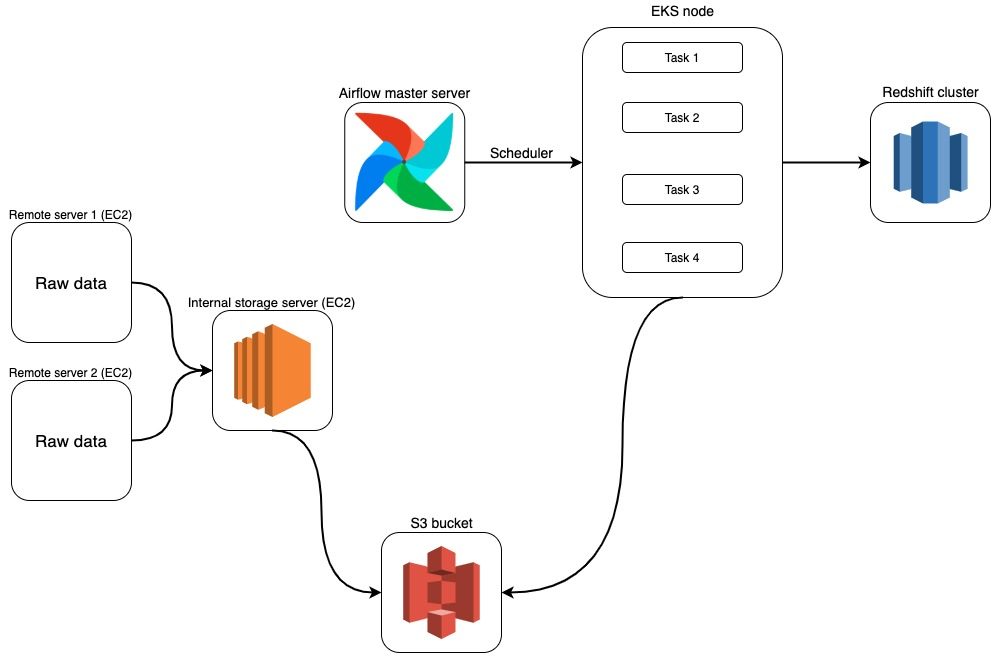
\includegraphics[width=14cm]{arch.jpg}
%	\caption{\label{arch}
%		Архитектура ETL процесса}
%\end{figure}

\begin{figure}[!ht]
	\centering
	\includegraphics[width=14cm]{arch_simple.jpg}
	\caption{\label{arch_simple}
		Архитектура ETL процесса}
\end{figure}

Ключевым элементом архитектуры является Apache Airflow, который запускает задачи обработки данных. Вся архитектура расположена в виртуальной частной сети, предоставленной AWS. Необработанные данные хранятся на отдельных инстансах (1, 2), которые моделируют источники данных. При запуске графа на Airflow инстансе (4) происходит проверка наличия данных на инстансах. Если данные присутствуют, начинается загрузка в S3 корзину (3) для их дальнейшей обработки. Затем запускается задача трансформации данных. Она выполняется в кластере EMR (7). Код программы для обработки написан с помощью фреймворка Spark на языке Python. Данная программа производит расчет метрик и конвертацию исходных файлов в формат Apache Parquet. Метрики сохраняются в хранилище данных Amazon Redshift (6), а файлы Parquet сохраняются в отдельную папку в S3 корзине (3).
Задачи Airflow запускаются на том же инстансе, где и сам Airflow, файл с описанием задач и логи выполнения хранятся в локальной файловой системе.
%Задачи Airflow запускаются в Kubernetes кластере (5), представленном в виде сервиса Amazon EKS (11). В качестве хранилища метаданных для Airflow используется инстанс базы данных, представленный сервисом Amazon RDS(6). Файл с описанием задач хранится в сетевой файловой системе Amazon EFS (9), а логи выполнения записываются в другую файловую систему того же типа (10).

\subsection{Серверы с необработанными данными}
Как было сказано ранее, серверы с необработанными данными являются EC2 инстансами типа t2.micro с  одним виртуальным ядром и 1Гб оперативной памяти. Инстансы используют дистрибутив Amazon Linux 2, основанный на дистрибутиве Red Hat Enterprise Linux компании Red Hat. Кроме стандартного пакета программ, на инстансы установлен Python интерпретатор версии 3.6, а также интерфейс коммандной строки AWS CLI, позволяющий управлять сервисами AWS прямо из командной строки. Это небходимо для копирования данных с сервера в S3 корзину. Необработанные данные хранятся в папке \verb|data/csv| и \verb|data/json| в домашней директории стандартного пользователя на каждом сервере соответственно.

\subsection{Среда запуска Spark приложений}
\subsubsection{Кластер}
Кластер для выполнения трансформации данных работает в сервисе AWS EMR. На кластере установлен фреймворк Apache Spark версии 2.4.4, а также в конфигурации добавлена поддержка Python третьей версии. Кластер состоит из двух узлов: одного главного узла и одного основного. Узлы являются инстансами типа m4.large с 4 виртуальными ядрами и 8Гб оперативной памяти, в качестве файловой системы кластера используется S3 корзина. Также при старте кластера на каждый узел будет установлен Python модуль boto3 с помощью, которого можно осуществить доступ к другим сервисам AWS из кода.

\subsubsection{Объектное хранилище}
В качестве файловой системы кластера и объектного хранилища для необработанный выступает S3 корзина. Все объекты в ней имеют класс хранения Standard. 
В корзине расположены следующие папки:
\begin{itemize}
	\item \verb|application| "--- содержит код Spark приложений;
	\item \verb|data| "--- соедржит необработанные данные, в ней есть 2 подпапки, csv и json, отвечающие за данные с разных серверов;
	\item \verb|dependencies| "--- папка с зависимостями для Spark приложения. В ней расположены \verb|.jar| файлы необходимых библиотек:
	\item \verb|emr-logs| "--- папка для логов. Все логи, производимые кластером записываются в эту папку;
	\item \verb|parquet| "--- папка, в которую сохраняются конвертированные файлы в формате  Parquet;
	\item \verb|tmp|"--- временная  папка для кэширования результатов записи в хранилище данных;
\end{itemize}

\subsubsection{Хранилище данных}
В качестве хранилища данных выступает кластер AWS Redshift. Кластер состоит из одного узла типа dc2.large с двумя виртуальными ядрами и 15Гб оперативной памяти, размер дискового пространства в кластере "--- 160Гб. В кластере была создана база данных \verb|metrics|, в которую записываются результаты работы Spark приложения. 

\subsection{Apache Airflow}
\subsubsection{Мастер сервер}
В качестве главного сервера на котором работает Airflow, выступает инстанс типа t3.medium с двумя виртуальными ядрами и 4Гб оперативной памяти. На сервер с помощью Ansible устанавливаются интерпретатор Python версии 3.6, интерфейс коммандной строки AWS CLI. Затем производится установка Airflow и создание рабочей директории для него, туда копируется файл конфигурации.
Также для возможности запуска задач в Kubernetes кластере устанавливается утилиты \verb|aws-iam-authenticator| и \verb|kubectl| и  производится их настройка. С их помощью и при правильной конфигурации Airflow сможет запускать задачи в Kubernetes.

\subsubsection{Хранилище метаданных}
В качестве хранилища метаданных для Airflow использует инстанс базы данных в сервисе AWS RDS типа db.t2.micro с 1 виртуальным ядром, 1Гб оперативной памяти и 10Гб дискового пространства.

\subsubsection{Kubernetes кластер}
\textbf{Docker} "--- программное обеспечение для автоматизации развертывания приложений в средах с поддержкой виртуализации. Позволяет переносить приложение со всеми зависимостями на любую Linux систему с поддержкой cgroups в ядре.

\textbf{Kubernetes}\ref{gigi} "--- платформа для автоматизации развертывания, управления и масштабирования контейнеров в кластере из серверов.
Основные концепции Kubernetes:
\begin{itemize}
	\item Кластер "--- набор серверов, хранилищ данных и сетевых ресурсов, с помощью которых Kubernetes запускает контейнеры в системе:
	\item Узел "--- это отдельный сервер, который запускает контейнеры. Каждый узел содержит в себе Kubernetes агент kubelet и прокси сервис;
	\item Ведущий узел "--- панель управления Kubernetes. Состоит из API"=сервера, планировщика и диспетчера контроллеров;
	\item Под "--- единица работы в Kubernetes. Каждый под содержит один или несколько контейнеров. Поды всегда работают совместно, то есть на одном сервере  Все контейнеры внутри пода имеют одни и те же IP"=адрес и пространство портов, они могут общаться между собой через локальный сервер или посредством межпроцессного взаимодействия. Кроме того, все контейнеры имеют доступ к обще- му локальному хранилищу данных узла, на котором находится под;
	\item Том "--- харнилище, которое может быть подключено к любому количеству контейнеров и не удаляется после удаления контейнеров. Существует различные типы томов для различных облачных платформ, сетевых файловых систем и Git репозиториев;
	\item Пространства имен "--- это виртуальный кластер. Один физический кластер может содержать несколько виртуальных, разделенных пространствами имен. Все виртуальные кластеры изолированы друг от друга, а общение происходит через публичные интерфейсы. 
	\item Запрос тома "--- запрос на доступ к тому для использования в поде;
\end{itemize}
\newpage

\section{Программная реализация}
%\subsection{Структура проекта}

\subsection{Скрипты создания инфраструктуры}
Для достижения большей гибкости при создании инфраструктуры и возможности переиспользования кода, Terraform позволяет параметризовать атрибуты ресурсов. С помощью конструкции \verb|variable|\ref{tf:var} Terraform позволяет задать переменную определенного типа и задать ей стандартное значение.
Пример конструкции \verb|variable|

\lstinputlisting[language=HCL]{example.tf}

В строке 2 указывается тип переменной, в данном случае это переменная строкового типа. В строке 3 указывается краткое описание этой переменной, а в строке 4 указывается стандартное значение.

Также для объединения и создания группы ресурсов Terraform поддерживает модульность. Модули, созданные другими разработчиками загружаются с помощью команды \verb|terraform get|\ref{tf:get}, также у Terraform есть конструкции \verb|data|\ref{tf:data} и \verb|output|\ref{tf:output}, которые позволяет хранить данные из других конфигураций или из внешних файлов и выводить необходимые данные в консоль после применения конфигурации.
Создание собственных модулей обычно предусматривает наличие трех файлов:
\begin{itemize}
	\item \verb|main.tf| "--- главный файл, в нем содержится вся конфигурация инфраструктуры;
	\item \verb|variables.tf| "--- файл, содержащий описание переменных;
	\item \verb|outputs.tf| "--- файл, содержащий конфигурацию выводов в консоль;
\end{itemize}
%\subsubsection{Airflow мастер"=сервер}
\subsubsection{Airflow сервер}
Для создания сервера был использован ресурс \verb|aws_instance|, который создает EC2 инстанс с необходимыми параметрами. Помимо создания инстанса необходимо создать правила для группы безопасности, чтобы разрешить входящий трафик на определенные сетевые порты. 

Листинг файла с переменными для Airflow сервера:
\lstinputlisting[language=HCL]{/Users/andryyyha/Documents/diploma/aws/airflow-master/variables.tf}

В переменной \verb|region| указан регион в котором будет создана инфраструктура, регион по умолчанию us"=east"=2. В переменной \verb|ami_id| указан номер образа операционной системы, которая будет запущена на инстансе. В перемнной \verb|instance_type| содержится информация о типе инстанса, который будет запущен, а в переменной \verb|availability_zone| указана зона доступности в которой будет запущен инстанс. Переменная \verb|security_groups| содержит список групп безопасности, которые будут прикреплены к инстансу.

Листинг файла с описанием конфигурации Airflow сервера:
\lstinputlisting[language=HCL]{/Users/andryyyha/Documents/diploma/aws/airflow-master/main.tf}

В строке 1 указан облачный провайдер, в котором будет создана инфраструктура,  в аттрибуте \verb|region| указан регион.

В строках 5, 14 и 23 создаются ресурсы для правил группы безопасности. Они прикрепляются в необходимой группе безопасности, которая указана в аттрибуте \verb|security_group_id|.  Аттрибуты \verb|from_port| и \verb|to_port| обозначают диапазон портов для которых разрешен входящий/исходящий трафик. Если порт один, эти аттрибуты принимают одинаковое значение Аттрибут \verb|protocol| определяет протокол для которого действует данное правило применяется, аттрибут \verb|security_group_id| определяет группу безопасности, к которой будет прикреплено данное правило. Порты 5432, 8080 и 2049 необходимы для того, чтобы сервер мог получать траффик от хранилища метаданных, пользователей Airflow веб"=сервера и сетевой файловой системы соответственно. 

Ресурс \verb|aws_instance| создает Airflow сервер.
Описание аттрибутов:
\begin{itemize}
	\item \verb|ami| "--- ID образа операционной системы;
	\item \verb|instance_type| "--- тип инстанса;
	\item \verb|availability_zone| "--- зона доступности;
	\item \verb|key_name| "--- название зарегистрированного SSH ключа для доступа к серверу посредством одноименного протокола;
	\item \verb|vpc_security_group_ids| "--- группы безопасности, прикрепленные к инстансу;
	\item \verb|associate_public_ip_address| "--- флаг, который указывает назначать ли инстансу публичный IP адрес;
	\item \verb|root_block_device| "--- составной аттрибут отвечающий за дисковое пространство инстанса. В аттрибуте \verb|volume_type| указывается тип диска, а в \verb|volume_size| его размер;
\end{itemize}

Также хотелось бы выделить составной аттрибут \verb|provisioner| (рус. поставщик), который позволяет запускать различные команды в зависимости от его типа. В данном случае после создания ресурса будет запущенна команда в локальном терминале. В строке 44 будет поставщик запустит скрипт, который будет в цикле подключаться к инстансу по SSH, пока тот не станет доступен. Как только это произойдет, поставщик на строке 50 запустит Ansible конфигурацию Airflow сервера.

\subsubsection{Кластер EMR и S3 корзина}
Для создания кластера для обработки данных и S3 корзины были использованы модули \verb|cloudposse/terraform-aws-emr-cluster|\ref{cloudposse:emr} и \verb|cloudposse/terraform-aws-s3-log-storage|\ref{cloudposse:s3}. 
Рассмотрим файл с переменными:
\lstinputlisting[language=HCL, firstline=7, lastline=71]{/Users/andryyyha/Documents/diploma/aws/emr/variables.tf}

Переменная \verb|vpc_id| хранит ID виртуальной частной сети, где будет запущен кластер, а \verb|subnet_id| "--- ID подсети. Переменные с префиксами \verb|core| и \verb|master| имеют одинаковое назначение для основного и главного типов узлов соответственно. Рассмотрим переменные для основного узла:
\begin{itemize}
	\item \verb|core_instance_type| "--- тип инстанса, который будет запущен;
	\item \verb|core_instance_count| "--- их количество, по умолчанию 1;
	\item \verb|core_instance_ebs_size| "--- размер диска для кадого узла;
	\item \verb|core_instance_ebs_type| "--- тип диска;
\end{itemize}

Листинг файла с описанием инфраструктуры:
\lstinputlisting[language=HCL]{/Users/andryyyha/Documents/diploma/aws/emr/main.tf}


\subsection{Пример Spark приложения}
\subsubsection{Подсчет метрик}
\subsubsection{Конвертация в Parquet}
\subsection{Скрипты транспортировки данных}
\subsection{Airflow DAG}
\subsection{Конфигурации}
\subsubsection{Общие тома для логов и DAGов}
\subsubsection{Kubeconfig}
\subsubsection{Конфигурацяи Airflow для Kubernetes кластера}
\subsubsection{Конфигурация Airflow}

% Раздел "Заключение"
\conclusion
Заключение
\bibliographystyle{gost780uv}
\bibliography{thesis}

\appendix
%\section{Java"=приложение для автоматизированных тестов серверной части}\label{api-test-app}
%\subsection{Класс ProfilePageTest}
%\VerbatimInput[fontsize=\small]{summerpractice/api-test/src/test/java/ru/summerpractice/ProfilePageTest.java}
%\subsection{Класс DataProviderProfile}
%\VerbatimInput[fontsize=\small]{summerpractice/api-test/src/main/java/ru/summerpractice/dataproviders/DataProviderProfile.java}

\end{document}
